\documentclass[paper=letter,11pt]{scrartcl}

\KOMAoptions{headinclude=true, footinclude=false}
\KOMAoptions{DIV=14, BCOR=5mm}
\KOMAoptions{numbers=noendperiod}
\KOMAoptions{parskip=half}
\addtokomafont{disposition}{\rmfamily}
\addtokomafont{part}{\LARGE}
\addtokomafont{descriptionlabel}{\rmfamily}
%\setkomafont{pageheadfoot}{\normalsize\sffamily}
\setkomafont{pagehead}{\normalsize\rmfamily}
%\setkomafont{publishers}{\normalsize\rmfamily}
\setkomafont{caption}{\normalfont\small}
\setcapindent{0pt}
\deffootnote[1em]{1em}{1em}{\textsuperscript{\thefootnotemark}\ }


\usepackage{amsmath}
\usepackage[varg]{txfonts}
\usepackage[T1]{fontenc}
\usepackage{graphicx}
\usepackage{xcolor}
\usepackage[american]{babel}
% hyperref is needed in many places, so include it here
\usepackage{hyperref}

\usepackage{xspace}
\usepackage{multirow}
\usepackage{float}


\usepackage{braket}
\usepackage{bbm}
\usepackage{relsize}
\usepackage{tcolorbox}

\def\ketY{\ensuremath{\ket {\Psi}}}
\def\iGeV{\ensuremath{\textrm{GeV}^{-1}}}
%\def\mp{\ensuremath{m_{\textrm{proton}}}}
\def\rp{\ensuremath{r_{\textrm{proton}}}}
\def\me{\ensuremath{m_{\textrm{electron}}}}
\def\aG{\ensuremath{\alpha_G}}
\def\rAtom{\ensuremath{r_{\textrm{atom}}}}
\def\rNucl{\ensuremath{r_{\textrm{nucleus}}}}
\def\GN{\ensuremath{\textrm{G}_\textrm{N}}}
\def\ketX{\ensuremath{\ket{\vec{x}}}}
\def\ve{\ensuremath{\vec{\epsilon}}}


\def\ABCDMatrix{\ensuremath{\begin{pmatrix} A &  B  \\ C  & D \end{pmatrix}}}
\def\xyprime{\ensuremath{\begin{pmatrix} x' \\ y' \end{pmatrix}}}
\def\xyprimeT{\ensuremath{\begin{pmatrix} x' &  y' \end{pmatrix}}}
\def\xy{\ensuremath{\begin{pmatrix} x \\ y \end{pmatrix}}}
\def\xyT{\ensuremath{\begin{pmatrix} x & y \end{pmatrix}}}

\def\IMatrix{\ensuremath{\begin{pmatrix} 0 &  1  \\ -1  & 0 \end{pmatrix}}}
\def\IBoostMatrix{\ensuremath{\begin{pmatrix} 0 &  1  \\ 1  & 0 \end{pmatrix}}}
\def\JThree{\ensuremath{\begin{pmatrix}    0 & -i & 0  \\ i & 0  & 0 \\ 0 & 0 & 0 \end{pmatrix}}} 
\def\JTwo{\ensuremath{\begin{bmatrix}    0 & 0 & -i  \\ 0 & 0  & 0 \\ i & 0 & 0 \end{bmatrix}}}
\def\JOne{\ensuremath{\begin{bmatrix}    0 & 0 & 0  \\ 0 & 0  & -i \\ 0 & i & 0 \end{bmatrix}}}
\def\etamn{\ensuremath{\eta_{\mu\nu}}}
\def\Lmn{\ensuremath{\Lambda^\mu_\nu}}
\def\dmn{\ensuremath{\delta^\mu_\nu}}
\def\wmn{\ensuremath{\omega^\mu_\nu}}
\def\be{\begin{equation*}}
\def\ee{\end{equation*}}
\def\bea{\begin{eqnarray*}}
\def\eea{\end{eqnarray*}}
\def\bi{\begin{itemize}}
\def\ei{\end{itemize}}
\def\fmn{\ensuremath{F_{\mu\nu}}}
\def\fMN{\ensuremath{F^{\mu\nu}}}
\def\bc{\begin{center}}
\def\ec{\end{center}}
\def\nus{$\nu$s}

\def\adagger{\ensuremath{a_{p\sigma}^\dagger}}
\def\lineacross{\noindent\rule{\textwidth}{1pt}}

\newcommand{\multiline}[1] {
\begin{tabular} {|l}
#1
\end{tabular}
}

\newcommand{\multilineNoLine}[1] {
\begin{tabular} {l}
#1
\end{tabular}
}



\newcommand{\lineTwo}[2] {
\begin{tabular} {|l}
#1 \\
#2
\end{tabular}
}

\newcommand{\rmt}[1] {
\textrm{#1}
}


%
% Units
%
\def\m{\ensuremath{\rmt{m}}}
\def\GeV{\ensuremath{\rmt{GeV}}}
\def\pt{\ensuremath{p_\rmt{T}}}


\def\parity{\ensuremath{\mathcal{P}}}

\usepackage{cancel}
\usepackage{ mathrsfs }
\def\bigL{\ensuremath{\mathscr{L}}}

\usepackage{ dsfont }



\usepackage{fancyhdr}
\fancyhf{}



\lhead{\Large 33-444} % \hfill Introduction to Particle Physics \hfill Spring 2022}
\chead{\Large Introduction to Particle Physics} % \hfill Spring 2022}
\rhead{\Large Spring 2022} % \hfill Introduction to Particle Physics \hfill Spring 2022}

\begin{document}
\thispagestyle{fancy}

\begin{center}
{\huge \textbf{Lecture 9}}
\end{center}

{\fontsize{14}{16}\selectfont


{\Large \underline{\textbf{Summary From Last Time}}}

Now lets imagine building interactions.  Add interaction Hamiltonian.

eg: an interaction where two particles come in and two particles go out:
\begin{figure}[h]
\centering
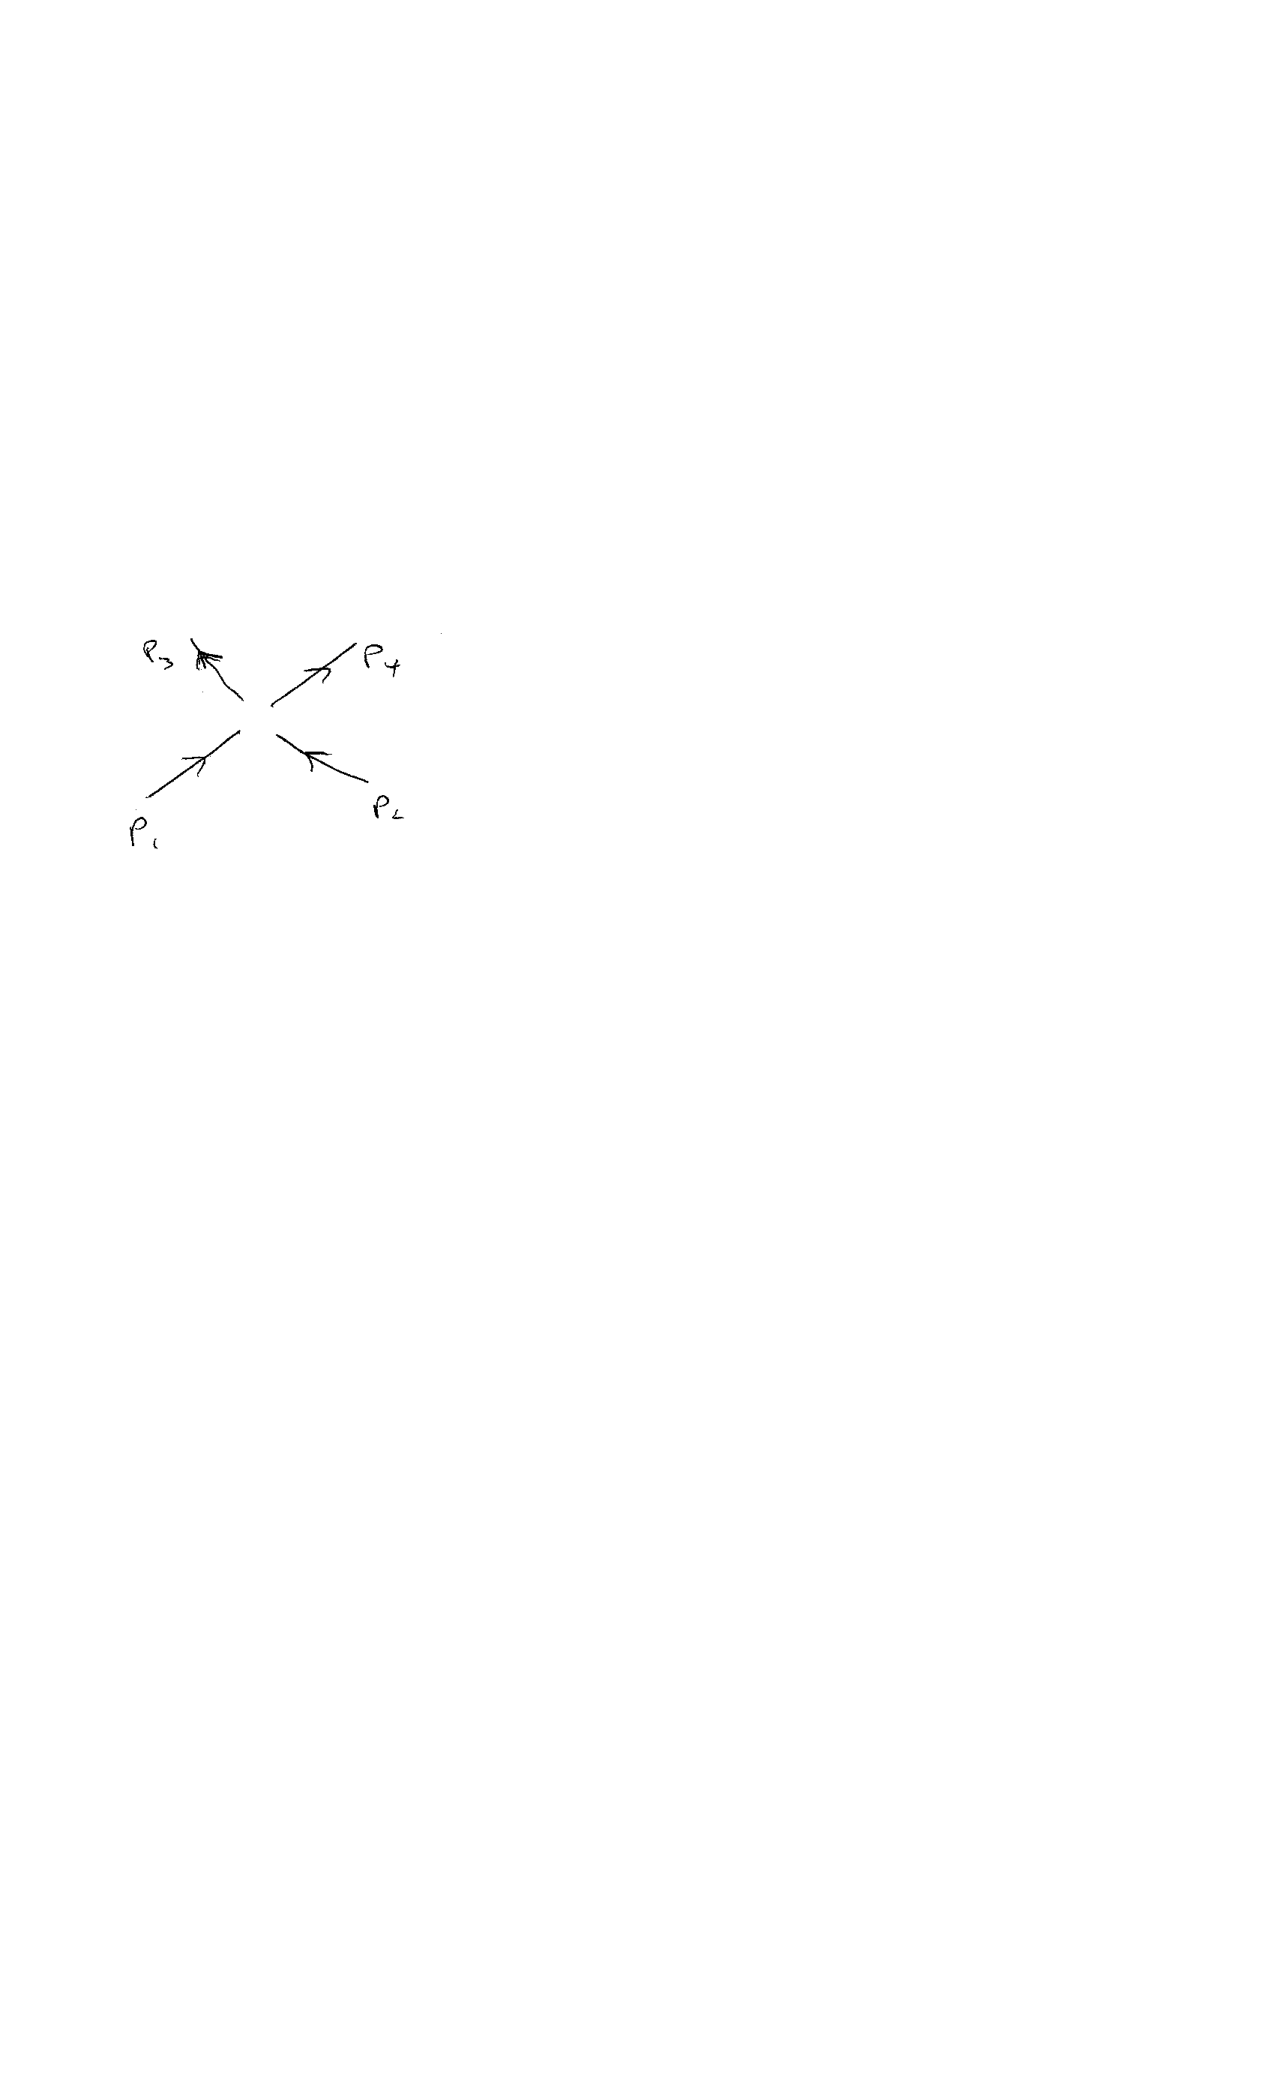
\includegraphics[width=0.4\textwidth]{./Interaction.pdf}
\end{figure}

This would correspond to adding an interaction term to the Hamiltonian of the form:

\bea
& \int \cancel{d}^3p_1 \cancel{d}^3p_2 \cancel{d}^3p_3 \cancel{d}^3p_4\ \delta(\vec{p_1}..\vec{p_4})\ \delta(E_1 + ... E_4) \\
& \underbrace{a^\dagger_{p_4,\sigma_4} a^\dagger_{p_3,\sigma_3} a_{p_2,\sigma_2} a_{p_1,\sigma_1} }_{\textrm{Acts on the initial state and gives the final state}} V(p's, \sigma's)   + \textrm{Hermitian Conjugate}
\eea

Interactions are made out of strings of a's and $a^\dagger$'s.
Also easy in this picture to talk about the creation and destruction of particles (Not just scattering) 

Very convenient to use this to map between particle states.

So far we have not said the word ``Field''. 

Now comes the challenge, 
\begin{itemize}
\item[-] These are interactions between momentum eigenstates
\item[-] Momentum Eigenstates are like big plane waves
\end{itemize}

A totally generic coefficient eg: ($\delta(\vec{p_1}..\vec{p_4}) \delta(E_1 + ... E_4) V(p's, \sigma's)$) is not going to correspond to point-like local interactions.\\

We would like to come up with some engine to allow us to build interaction Hamiltonians where we can just see explicitly that the interactions are local. 
\bi
\item[-]This is where the utility of the field concept comes in. \\
\ei

The states that we have defined act nicely under the translations operator (just pick up a phase) but to get interactions local in space we need x to make an appearance. 
That is, we want to build operators out of things like $\phi(\vec{x})$, where under T:$\phi(\vec{x}) \rightarrow \phi(\vec{x}+\vec{a})$


There is a very nice way of doing this called Fourier Transforms. 

\underline{Define}   

\be
\phi_+ (\vec{x}) = \int \cancel{d}^3p\ a^{\dagger}_{\vec{p}}\ e^{-i \vec{p} \vec{x}}
\ee

and

\be
\phi_- (\vec{x}) = \int \cancel{d}^3p\ a_{\vec{p}}\ e^{+i \vec{p} \vec{x}}
\ee

Note: $\phi_- (\vec{x}) = \phi^\dagger_+ (\vec{x})$

Indeed the $\phi$'s behave as above under translations.

\noindent\rule{\textwidth}{1pt}

Can now go back to the free Hamiltonian and write it very simply using the $\phi$'s.


$\textrm{H}^{\textrm{free}}$ (non-relativistic for the moment) $E_p = p^2/2m$

\be
\textrm{H}^{\textrm{free}} = \int d^3x\ \frac{(\vec{\nabla} \phi_+ )^\dagger (\vec{\nabla} \phi_+ )}{2m}
\ee
n
which is the same as 

\be
H = \sum\limits_{p,\sigma} E_p\ a^\dagger_{p,\sigma} a_{p,\sigma}
\ee


Now its clear how you could write down interactions that take place locally:

\be
\textrm{H}^{\textrm{free}} + \int d^3x\ C[\phi_+(x)\phi_+(x)\phi_-(x)\phi_-(x)] + ... 
\ee

Its totally clear now that this is local is space. 

Taking this an expanding out gives something like we just talked about with 2a's and 2 $a^\dagger$'s.
All the rest comes along for the ride. 

(Note that this is all done non-relativistically for the moment to stress that this has nothing to do w/relativity.
This is about making interactions local)

Why we use fields: Makes local interactions of \underline{particles} manifest.

Locality is hardwired into the descriptions of particles.

So, where does relativity come in?  Where is the difficulty ?

\underline{Time Evolution}

\begin{figure}[h]
\centering
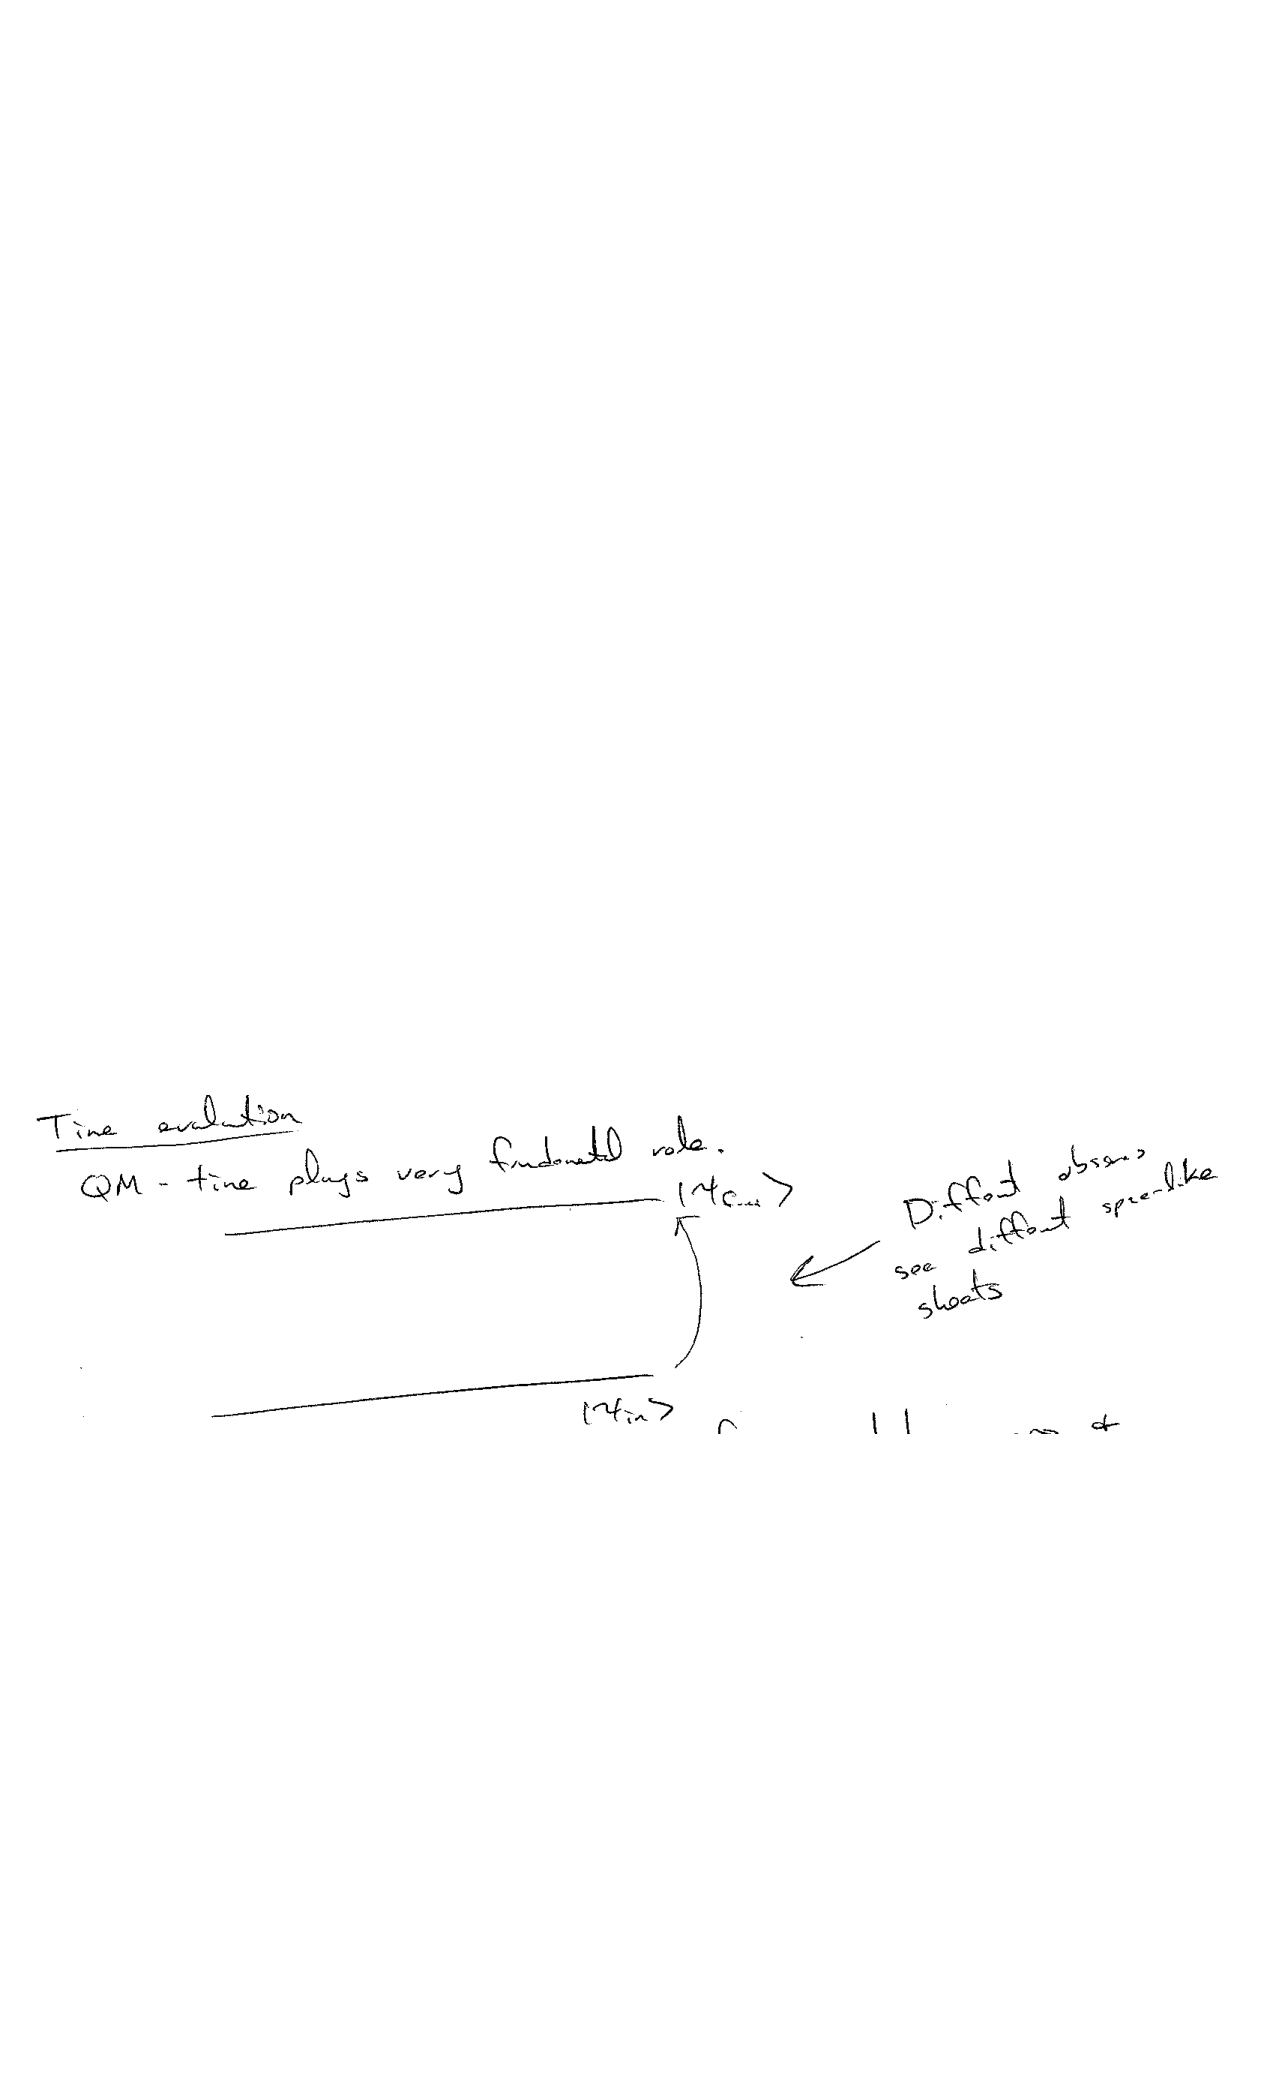
\includegraphics[width=0.9\textwidth]{./TimeEvolution.pdf}
\end{figure}

Only have a hope of Lorentz invariance if we start at -$\infty$ and go to +$\infty$.

Throw particles in from $\infty$ let them scatter \& go back out to $\infty$.

\underline{Define S-Matrix}

\be
\underbrace{\ket{p_1 \sigma_1,...p_n\sigma_n}}_{t=-\infty} \rightarrow \underbrace{\mathcal{S} \ket{p_1\sigma_1,...p_n\sigma_n}}_{t=+\infty}
\ee

$\mathcal{S}$ might be (at least a hope) Lorentz Invariant.

\noindent\rule{\textwidth}{1pt}

\textbf{Big Picture:}
The plan is to Figure out what $\mathcal{S}$ is in a totally generic theory, then see what it would take to make it Lorentz Invariant. 

Sure doesn't look like it will be L.I. 
$\mathcal{S}$ is the only object that you could even have a hope to make L.I.

We will see that for \underline{very special} choices of the interaction it will barely be possible for it to be Lorentz Invariant. 
These choices force on us anti-particle and the connection between spin and statistics. 

\noindent\rule{\textwidth}{1pt}

Something annoying that we should get rid of right away. 
Free evolution, just evolves w/phase. Totally irrelevant part.


Standard way of removing the free evolution \underline{``Interaction Representation''}.

\be
H = H_\textrm{free} + H_\textrm{Int}
\ee


\be
i \frac{d \ket{\psi}}{d t} = \left(H_\textrm{free} + H_\textrm{Int} \right) \ket{\psi} 
\ee

\underline{For $H_\textrm{Int}$ = 0}

\be
\ket{\psi} = e^{-i H_f t} \ket{\psi_{in}}
\ee

Now, we don't have a free theory, but if the interaction is small going to be pretty close to evolving like this. 


\begin{equation}\label{eq:def}
\ket{\psi} = e^{-i H_f t} \underbrace{\ket{\psi_{I}}}_{\textrm{definition}}
\end{equation}

If $H_\textrm{Int} = 0, \ket{\psi_\textrm{Int}}$ doesn't evolve at all.
Bc there is $H_\textrm{Int}$, $\ket{\psi_\textrm{Int}}$ will evolve. 

\bea
i \frac{d }{d t} \ket{\psi} &=& H_\textrm{f} \ket{\psi} + e^{-i H_f t} i \frac{d }{d t} \ket{\psi_I} \\
&=& (H_f + H_\textrm{int}) e^{-i H_f t} \ket{\psi_I}
\eea

Note: first line from derivative of~\ref{eq:def}, the second from the Schrodinger Equation.

The RHSs imply, 

\be
i \frac{d }{d t} \ket{\psi_I} =  \underbrace{e^{+i H_f t} H_\textrm{Int} e^{-i H_f t}}_{\textrm{Interaction Hamiltonian in the interaction representation}}  \ket{\psi_I} 
\ee


So, 

\be
i \frac{d }{d t} \ket{\psi_I} =  H_I  \ket{\psi_I} 
\ee
where $H_I$ can be time dependent. 

\underline{Lets formally solve this} 

Just integrating gives,

\be
\ket{\psi_I (t_2)} = \ket{\psi_I (t_1)} - i \int_{t_1}^{t_2} dt H_I \ket{\psi_I(t)}
\ee

Now we can keep iterating, 

\be
 = \ket{\psi_I (t_1)} - i \int_{t_1}^{t_2} dt H_I(t) \left( \ket{\psi_I (t_1)} - i \int_{t_1}^{t} dt' H_I(t') \ket{\psi_I(t')}\right)
\ee

or

\be
 = \ket{\psi_I (t_1)} - i \int_{t_1}^{t_2} dt H_I \ket{\psi_I (t_1)}  +  (-i)^2 \int_{t_1}^{t_2} dt \int_{t_1}^{t} dt' H_I(t)H_I(t')\ket{\psi_I(t')}
\ee

Pattern is clear,  can keep going...

\bea
\ket{\psi_I (t_2)} = [ &1& + (-i) \int_{t_1}^{t_2} dt H_I(t) \\
    &+& (-i)^2 \int_{t_1}^{t_2} dt \int_{t_1}^{t} dt' H_I(t)H_I(t') \\
    &+&  (-i)^3 \int_{t_1}^{t_2} dt \int_{t_1}^{t} dt' \int_{t}^{t'} dt'' H_I(t) H_I(t') H_I(t''') \\
    &+& ...  ] \ket{\psi_I (t_1)}
\eea

If $H_I$ is small this is giving us some nice perturbation theory. 

\begin{figure}[h]
\centering
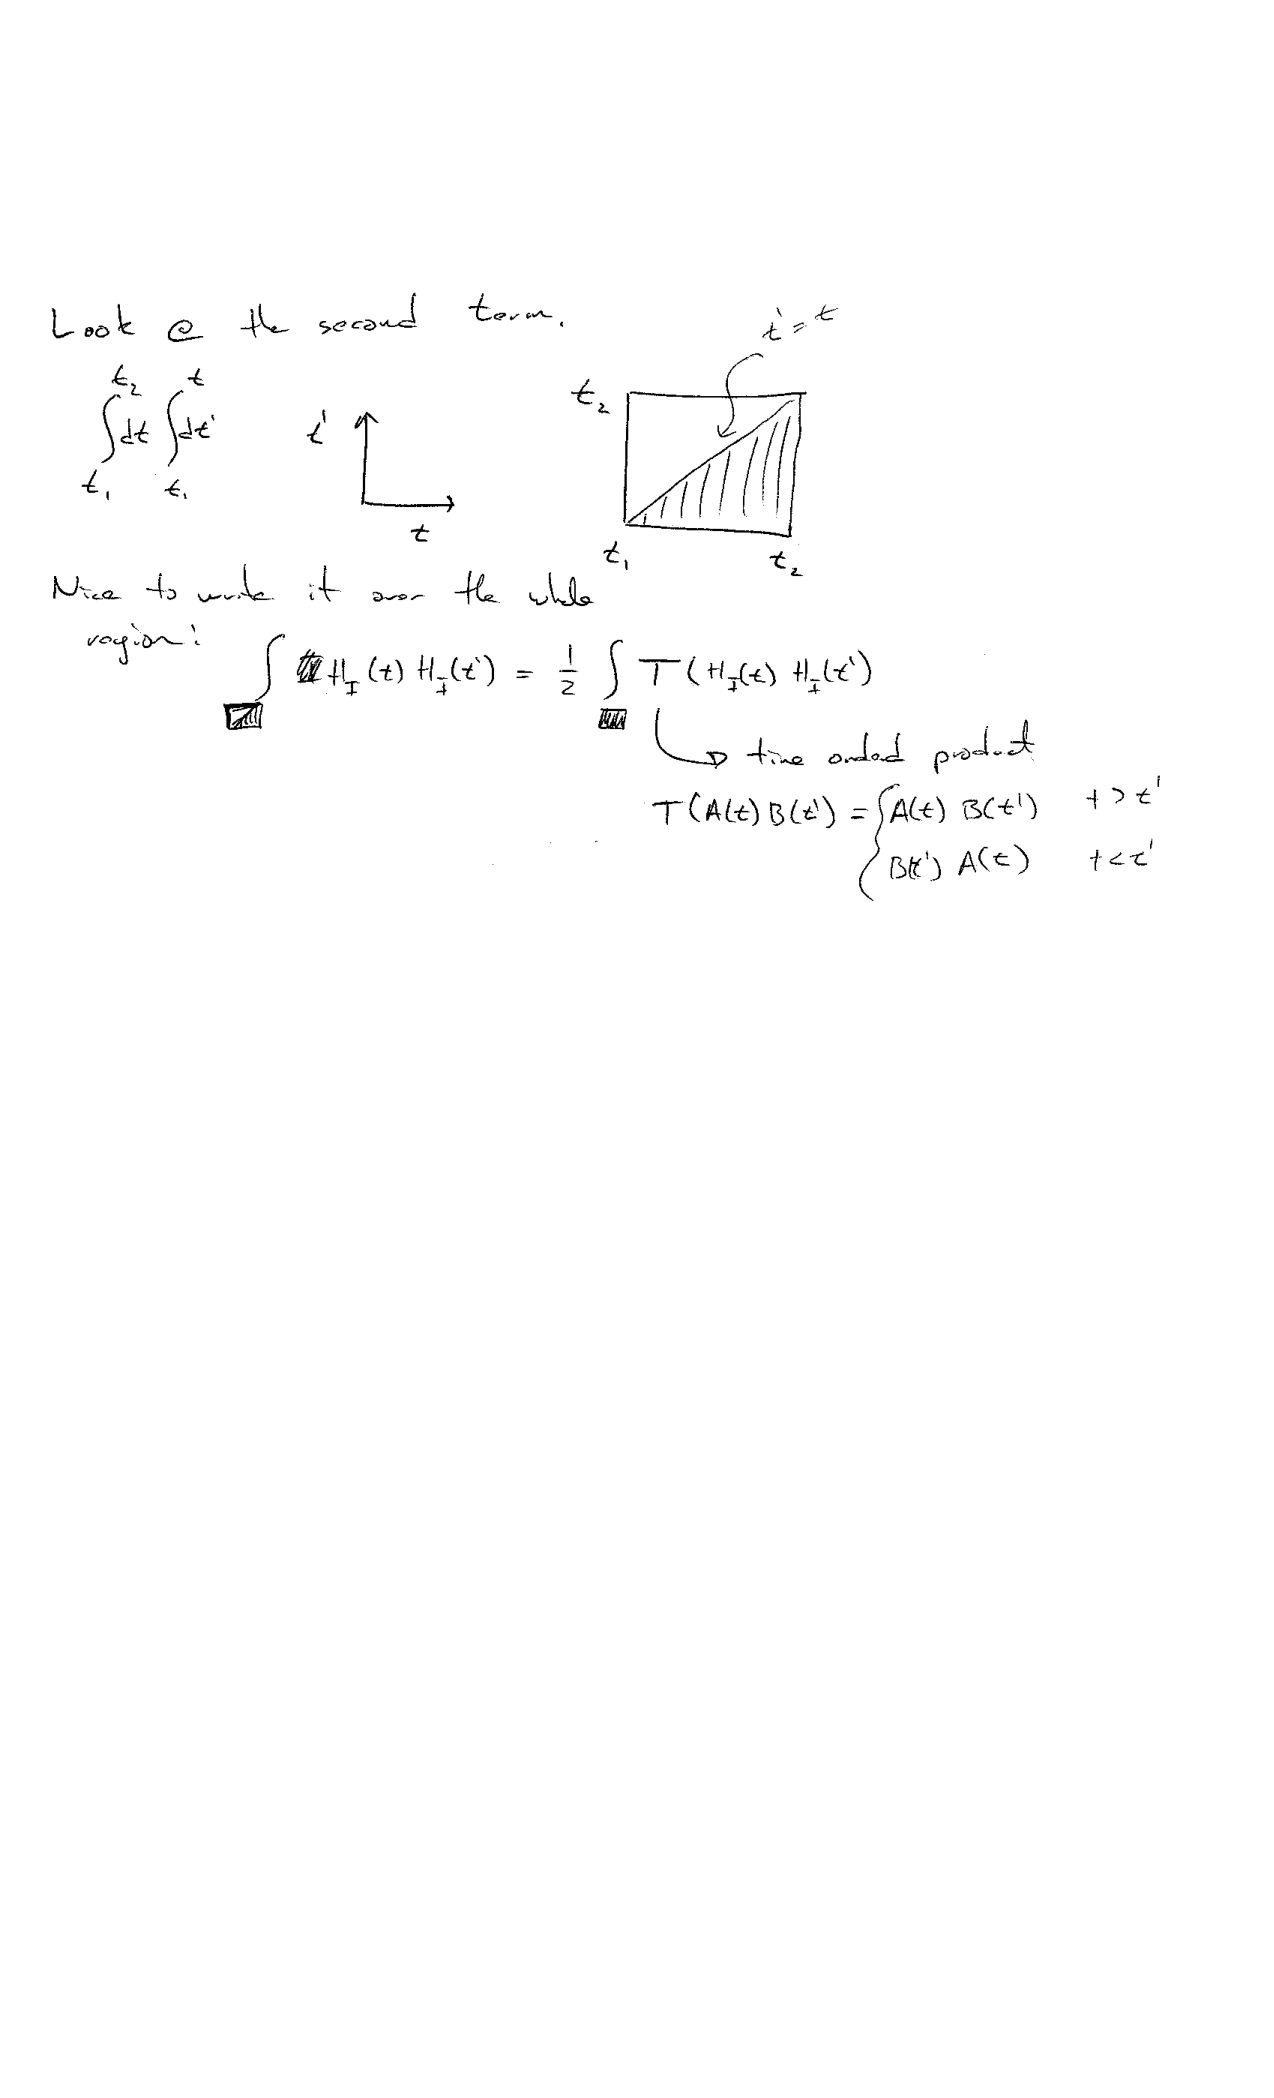
\includegraphics[width=0.9\textwidth]{./IntegrationLimits.pdf}
\end{figure}


\bea
\ket{\psi_I (t_2)} = [ &1& + (-i) \int_{t_1}^{t_2} dt \top(H_I(t)) \\
    &+& \frac{(-i)^2}{2!} \int_{t_1}^{t_2} dt \int_{t_1}^{t} dt' \top(H_I(t)H_I(t')) \\
    &+&  \frac{(-i)^3}{3!} \int_{t_1}^{t_2} dt \int_{t_1}^{t} dt' \int_{t}^{t'} dt'' \top(H_I(t) H_I(t') H_I(t''')) \\
    &+& ...  ] \ket{\psi_I (t_1)}
\eea


\be
\ket{\psi_I (t_2)} = \top\left( e^{ (-i) \int_{t_1}^{t_2} dt H_I(t)} \right)\ket{\psi_I (t_1)}
\ee

Now, let $t_1$ and $t_2$ go to $\infty$,


\be
\ket{\psi_I (+\infty)} = \top\left( e^{ (-i) \int_{-\infty}^{+\infty} dt H_I(t)} \right)\ket{\psi_I (-\infty)}
\ee

OK, Lets go back to field theory....

\noindent\rule{\textwidth}{1pt}

\be
\phi_+ (\vec{x}) = \int \cancel{d}^3p\ e^{-i \vec{p} \vec{x}}\ a^{\dagger}_{\vec{p}}
\ee

(use scalars for the moment) 

Need to build $H_I$ out of $\phi_{+/-}$ in the interaction representation.

\fbox{\begin{minipage}{\textwidth}
Note: 
\be
\phi_+^I (x, t) = e^{+iH_ft} \phi(x) e^{-iH_ft} \rightarrow e^{iE_p t} \phi(x) \\
\ee


The $e^{-iHt}$ will go to $e^{-iEt}$, then $\phi(x)$ will create a new particle with energy $E_p$, and then the $e^{+iHt}$ will give $e^{i(E+E_p) t}$

\end{minipage}}



}
\end{document}


